\documentclass[11pt]{article}
\usepackage{../style/forage}
\usepackage{needspace}
\usetikzlibrary{positioning}

% Figures and tables in figures/ are generated by analysis.ipynb.
% Re-run the notebook if the assumptions change, then recompile.

% keep headings with the text that follows them
\let\oldsubheading\subheading
\renewcommand{\subheading}[1]{\Needspace{6\baselineskip}\oldsubheading{#1}}
\let\oldheading\heading
\renewcommand{\heading}[1]{\Needspace{8\baselineskip}\oldheading{#1}}

% one row of the before/after workflow diagram
\newcommand{\flowrow}[6]{% {label}{colour}{s1}{s2}{s3}{s4}
  \begin{tikzpicture}[
      box/.style={fill=#2, text=white, text width=2.75cm, minimum height=1.55cm,
        align=center, font=\footnotesize, inner sep=1.5mm},
      arr/.style={-latex, thick, color=gray}]
    \node[font=\small\bfseries, text width=1.9cm, align=left] (l) at (-6.9,0) {#1};
    \node[box] (a) at (-4.6,0) {#3};
    \node[box] (b) at (-1.4,0) {#4};
    \node[box] (c) at (1.8,0) {#5};
    \node[box] (d) at (5.0,0) {#6};
    \draw[arr] (a) -- (b); \draw[arr] (b) -- (c); \draw[arr] (c) -- (d);
  \end{tikzpicture}}

\begin{document}

% ================= Title page =================
\begin{titlepage}
  \vspace*{4cm}
  {\color{navy}\fontsize{30}{36}\selectfont Process Improvement\\[2mm]
  Proposal}\par\medskip
  {\Large From 90 Minutes to Under 10:\\
  Automating Apex Global Investments' Trade Execution Workflow}\par
  {\color{rulegray}\rule{\linewidth}{0.6pt}}\par\bigskip
  \begin{tabular}{@{}ll}
    \textbf{Proposal Title:} & Process Improvement Proposal for Apex Global
                               Investments \\
    \textbf{Prepared by:}    & Thiziri Amezza, Sales and Trading Analyst \\
    \textbf{Date:}           & \today \\
    \textbf{Client:}         & Apex Global Investments \\
  \end{tabular}
  \vfill
  {\small\color{gray}Prepared as part of the Bank of America Global Markets
  Sales and Trading job simulation (Forage). Hypothetical client. Workflow
  times, error rate and missed-opportunity figures come from the Client
  Profile Reference Sheet; the performance of automated steps and the costs
  are stated assumptions. All figures and tables are reproducible with
  \texttt{analysis.ipynb}.}
\end{titlepage}

% ================= At a glance =================
\heading{Proposal at a Glance}
\infobox{\faBolt}{Summary}{
  \item \textbf{Problem:} three manual hand-offs (data entry, cross-system
  validation and compliance approval) make every trade wait about
  \textbf{60 minutes} before it can be executed. A further 30 minutes go on
  the manual report. Reconciliation errors affect \textbf{12\%} of trades,
  and delays cost an estimated \textbf{\$500,000 last quarter}.
  \item \textbf{Solution:} a reconciliation engine, automated reports,
  rule-based compliance pre-checks and automated trade capture, rolled out in
  three phases over 16 weeks.
  \item \textbf{Impact (simulated):} average time to execution falls from
  about \textbf{63 to 6 minutes} (\textminus90\%); the error rate falls from
  \textbf{12\% to about 2\%}.
  \item \textbf{Investment:} about \$400k in year one. The payback period is
  between 3 and 11 months, depending on how much of the time saved is
  recovered as trading opportunities.
}

% ================= Section 1 =================
\heading{1. Summary of Identified Issue}

\subheading{Workflow Analyzed}
The \textbf{trade execution process}: from the moment trade details are
captured until the trade summary reaches stakeholders. Today, each of its four
steps is carried out by hand.

\begin{center}
\flowrow{Today\\(90 min)}{navy}{Data entry\\[1mm]\textit{manual, $\sim$15
min}}{Cross-system validation\\[1mm]\textit{manual, $\sim$20 min}}{Compliance
approval\\[1mm]\textit{manual, $\sim$25 min}}{Report generation\\[1mm]\textit{manual,
$\sim$30 min}}\par\medskip
\flowrow{Proposed\\($<$10 min)}{correctgreen}{Automated trade
capture\\[1mm]\textit{API, $\sim$1 min}}{Reconciliation engine\\[1mm]\textit{exceptions
only, $\sim$2 min}}{Rule-based pre-checks\\[1mm]\textit{officer sees
exceptions}}{Automated report\\[1mm]\textit{template, $\sim$2 min}}\par
{\small\color{gray}Figure 1 --- Current and proposed trade execution
workflow. Times from the Client Profile Reference Sheet.}
\end{center}

\subheading{Identified Bottleneck}
The bottleneck is not one step. It is the \textbf{chain of manual hand-offs
that must be completed before a trade can be executed}:
\begin{itemize}[leftmargin=1.5em, itemsep=2pt]
  \item \textbf{Compliance approval ($\sim$25 min)} is the longest pre-trade
  step. Every trade waits for a compliance officer, including routine trades
  that clearly meet the rules.
  \item \textbf{Cross-system validation ($\sim$20 min)} is where errors
  originate. Comparing data across two systems by hand produces the
  \textbf{12\% reconciliation error rate}, and each error sends the trade back
  through validation and compliance.
  \item \textbf{Data entry ($\sim$15 min)} re-types information that already
  exists in electronic form, which creates the errors validation then has to
  catch.
\end{itemize}
Report generation (30 min) is the longest single step, but it happens after
execution: it delays stakeholders, not the trade.

\subheading{Impact on Client Goals}
\begin{itemize}[leftmargin=1.5em, itemsep=2pt]
  \item \textbf{Speed:} for a high-frequency trading client, a 60-minute wait
  before execution means trading on prices that may no longer be there. Apex
  estimates \textbf{\$500,000 of missed opportunities last quarter}, or about
  \$2 million a year at the current rate.
  \item \textbf{Accuracy:} a 12\% error rate weakens reporting accuracy and
  adds risk, which goes against Apex's objective to ``mitigate risks
  associated with manual reconciliation''.
  \item \textbf{Growth:} the process cannot scale. More volume means
  proportionally more manual work and more errors.
\end{itemize}
\textbf{Why now:} market conditions currently suit Apex's strategy, so every
delayed trade is a lost opportunity.

% ================= Section 2 =================
\heading{2. Proposed Solution}

\subheading{Recommended Improvements}
\begin{enumerate}[leftmargin=1.5em, itemsep=4pt]
  \item \textbf{Automated reconciliation engine.} A rule-based tool matches
  trades across the two systems automatically (same trade ID, price, quantity
  and date within set tolerances). Analysts see only the exceptions it flags,
  not every line.
  \item \textbf{Automated report generation.} A template pulls the reconciled
  data, builds the trade summary with its charts and distributes it on a
  schedule. This is the same approach used to produce the reports in earlier
  parts of this project.
  \item \textbf{Rule-based compliance pre-checks.} Apex's compliance team
  encodes its standards as rules: position limits, restricted lists, trade
  size and counterparty checks. Trades that pass all rules are approved
  automatically and logged for audit. The compliance officer reviews only the
  trades that are flagged (we assume about 15\%).
  \item \textbf{Automated trade capture.} An API connection sends trade
  details straight from the order system into the internal systems,
  removing manual data entry and the errors it creates.
\end{enumerate}

\subheading{Connection to Client Goals}
\begin{center}
\small
\begin{tabular}{@{}p{5.2cm}p{10.6cm}@{}}
  \toprule
  \textbf{Apex objective} & \textbf{How the solution delivers it} \\
  \midrule
  Optimize trade execution for speed and accuracy & Time to execution falls by
    about 90\%; the error rate falls from 12\% to about 2\%. \\
  Mitigate risks of manual reconciliation and data handling & Data is no
    longer re-typed; matching is rule-based, consistent and logged. \\
  Align processes with high-growth market opportunities & Trades are executed
    while opportunities are still available; the process scales with volume
    instead of headcount. \\
  \bottomrule
\end{tabular}
\end{center}

% ================= Section 3 =================
\heading{3. Justification for Solution}

\subheading{Why This Solution?}
\begin{itemize}[leftmargin=1.5em, itemsep=2pt]
  \item \textbf{It targets the root cause, not the symptom.} Adding staff
  would shorten queues but keep the manual errors. Automation removes both
  the waiting and the error source.
  \item \textbf{Compliance stays in control.} Officers define the rules, keep
  an audit trail of every automatic approval, and spend their time on the
  trades that really need judgement.
  \item \textbf{It fits limited IT resources.} The rollout starts with tools
  that run on data Apex already exports (reconciliation and reporting), and
  leaves the deeper API integration for last, managed by the vendor.
  \item \textbf{Every phase pays off on its own.} Each phase can be measured
  before the next one is approved, as Apex's leadership requires (``if the
  benefits outweigh the costs'').
\end{itemize}

\subheading{Supporting Evidence}
We simulated 10,000 trades through the current and the automated workflow,
using the step times and error rate from the Client Profile Reference Sheet.

\begin{center}
  \small\begin{tabular}{@{}lrrr@{}}
\toprule
\textbf{Metric (10{,}000 simulated trades)} & \textbf{Current} & \textbf{Automated} & \textbf{Change} \\
\midrule
Average time to execution (min) & 62.7 & 6.3 & \textminus{}90\% \\
Slowest 5\% of trades: time to execution (min) & 86.8 & 20.1 & \textminus{}77\% \\
End-to-end time incl.\ report (min) & 92.7 & 8.3 & \textminus{}91\% \\
Reconciliation error rate (\%) & 12.1 & 1.9 & \textminus{}84\% \\
\bottomrule
\end{tabular}\par\smallskip
  {\color{gray}Table 1 --- Simulation results. ``Time to execution'' covers
  the three pre-trade steps, including error rework.}
\end{center}

\begin{center}
  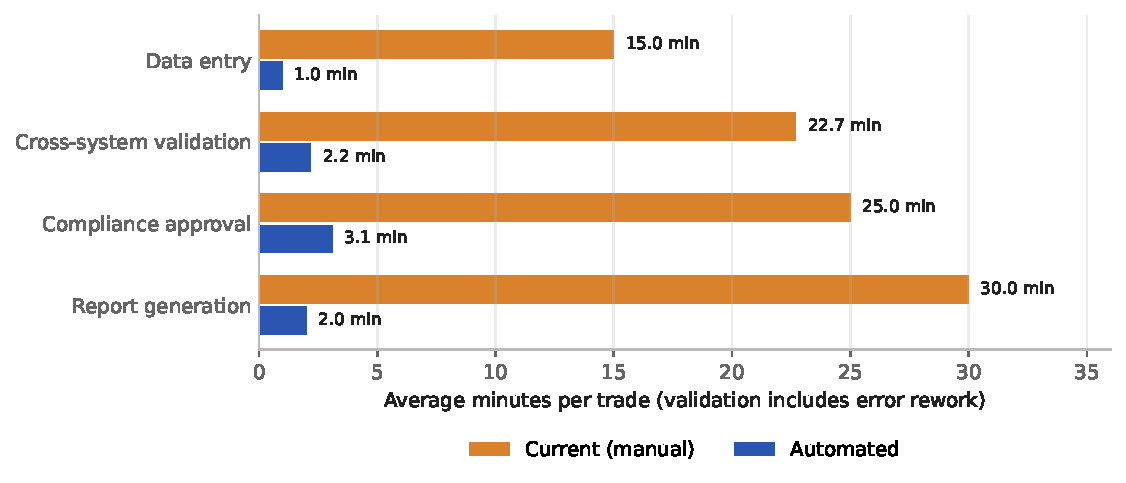
\includegraphics[width=0.88\linewidth]{figures/fig1_step_times.pdf}\par
  {\small\color{gray}Figure 2 --- Average minutes per step, current vs.\
  automated.}
\end{center}

\begin{center}
  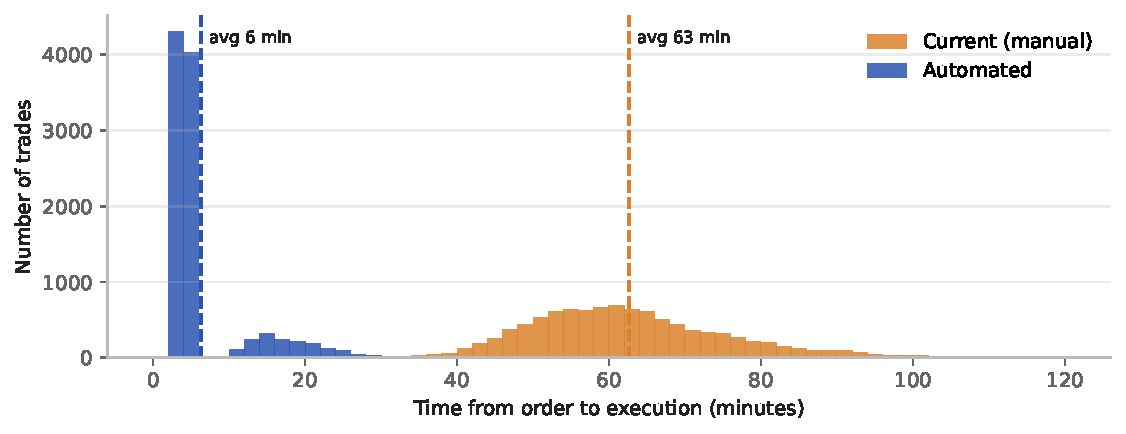
\includegraphics[width=0.88\linewidth]{figures/fig2_distribution.pdf}\par
  {\small\color{gray}Figure 3 --- Distribution of time to execution across
  10,000 simulated trades. The small second group of automated trades shows
  the exceptions sent to a compliance officer.}
\end{center}

These results are consistent with earlier findings in this project: in the
workflow analysis exercise, manual comparison of confirmations and manual
compliance approval were identified as the steps with the highest risk of
delay.

% ================= Section 4 =================
\heading{4. Implementation Plan}

\subheading{Steps to Implement}
\begin{center}
\small
\begin{tabular}{@{}p{3.4cm}p{1.9cm}p{10.4cm}@{}}
  \toprule
  \textbf{Phase} & \textbf{Timing} & \textbf{Actions} \\
  \midrule
  \textbf{1. Quick wins} & Weeks 1--6 & Deploy the reconciliation engine on the
    two systems' existing exports and set matching tolerances. Pilot it on the
    Technology book (50\% of the portfolio), then extend it. Switch report
    generation to an automated template. \\
  \textbf{2. Compliance rules} & Weeks 5--10 & With the compliance team, write
    the pre-check rules. Run them in parallel with manual approval for two
    weeks and compare the decisions, then switch to automatic approval with
    exception review. \\
  \textbf{3. Trade capture} & Weeks 9--16 & Vendor-managed API connection from
    the order system to the internal systems. Run it in parallel with manual
    entry until match rates are confirmed. \\
  \textbf{Training} & Throughout & Short sessions for analysts (handling
    exceptions) and compliance (maintaining rules); written runbooks. \\
  \bottomrule
\end{tabular}
\end{center}

\begin{center}
  \small\begin{tabular}{@{}lrrr@{}}
\toprule
\textbf{Stage} & \textbf{Time to execution} & \textbf{End-to-end} & \textbf{Error rate} \\
\midrule
Today (manual) & 63 min & 93 min & 12.1\% \\
Phase 1: reconciliation engine + auto reports & 42 min & 44 min & 1.9\% \\
Phase 2: + rule-based compliance pre-checks & 20 min & 22 min & 2.1\% \\
Phase 3: + automated trade capture (API) & 6 min & 8 min & 1.8\% \\
\bottomrule
\end{tabular}\par\smallskip
  {\color{gray}Table 2 --- Simulated average times and error rate after each
  phase.}
\end{center}

\subheading{Required Tools and Resources}
\begin{itemize}[leftmargin=1.5em, itemsep=2pt]
  \item \textbf{Tools:} a reconciliation and matching tool, a reporting tool
  with templates (or Python scripts), a compliance rules engine with audit
  logging, and an API connection to the order system.
  \item \textbf{People (from Apex's existing roles):} a \emph{Project
  Manager} for timeline and coordination; an \emph{IT Specialist} for the
  integrations, supported by the vendor to offset limited IT capacity;
  \emph{Compliance Officers} to define and approve rules; a \emph{Data
  Analyst} to set matching tolerances and handle exceptions; and a \emph{Risk
  Management Specialist} to monitor exception trends.
\end{itemize}

% ================= Section 5 =================
\heading{5. Expected Outcomes}

\subheading{Benefits}
\begin{itemize}[leftmargin=1.5em, itemsep=2pt]
  \item \textbf{Speed:} average time to execution falls from about 63 to about
  6 minutes, and from about 87 to about 20 minutes for the slowest 5\% of
  trades.
  \item \textbf{Accuracy:} the reconciliation error rate falls from 12\% to
  about 2\%, and the remaining exceptions are flagged automatically rather
  than found late.
  \item \textbf{Capacity:} analysts and compliance officers spend their time
  on exceptions, analysis and clients instead of re-typing and comparing
  data.
  \item \textbf{Client satisfaction:} faster, more reliable execution and
  same-day reporting.
\end{itemize}

\subheading{Cost and Benefit}
\begin{center}
  \small\begin{tabular}{@{}lrrrr@{}}
\toprule
\textbf{Scenario} & \textbf{Annual benefit} & \textbf{Year-1 net} & \textbf{Payback} & \textbf{3-year net} \\
\midrule
25\% of time saved is recovered & \$450k & \$50k & 10.7 months & \$709k \\
50\% of time saved is recovered & \$899k & \$499k & 5.3 months & \$2,057k \\
100\% of time saved is recovered & \$1,798k & \$1,398k & 2.7 months & \$4,755k \\
\bottomrule
\end{tabular}\par\smallskip
  {\color{gray}Table 3 --- Illustrative cost--benefit, based on \$2.0m a year
  of missed opportunities at today's rate, a 90\% cut in time to execution,
  \$400k year-one cost and \$120k a year after that.}
\end{center}
Even in the most conservative case, where only a quarter of the time saved
turns into recovered opportunities, the project pays back within about a year.

\subheading{Metrics for Success}
\begin{center}
\small
\begin{tabular}{@{}lrr@{}}
  \toprule
  \textbf{Metric} & \textbf{Today} & \textbf{Target (after Phase 3)} \\
  \midrule
  Average time to execution & $\sim$60 min & $<$10 min \\
  Trade execution time, end to end & 90 min & $<$15 min \\
  Reconciliation error rate & 12\% & $<$3\% \\
  Share of trades approved automatically & 0\% & $\geq$80\% \\
  Missed opportunities due to delays & $\sim$\$500k / quarter & $-$50\% within
    two quarters \\
  \bottomrule
\end{tabular}
\end{center}
We suggest reviewing these metrics weekly during the rollout and monthly
afterwards.

% ================= Section 6 =================
\heading{6. Conclusion}

\subheading{Final Recommendation}
Apex's trades are slowed by manual hand-offs, not by the market. Automating
reconciliation, reporting, routine compliance checks and trade capture
targets the cause of both the delays and the errors. In our simulation it
cuts time to execution by about 90\% and the error rate from 12\% to about
2\%. The phased plan keeps compliance in control, respects Apex's limited IT
capacity, and pays back within a year even under cautious assumptions.

\subheading{Call to Action}
We recommend approving Phase 1 now. It can start within a week, needs little
integration work, and will deliver measurable results within six weeks to
inform the decision on Phases 2 and 3. We would be glad to meet your
operations, compliance and IT leads this week to agree on the pilot scope.

% ================= Appendix =================
\heading{Appendix --- Simulation Method and Assumptions}
\begin{itemize}[leftmargin=1.5em, itemsep=3pt]
  \item \textbf{From the profile sheet:} step means of 15 / 20 / 25 / 30
  minutes, a 12\% reconciliation error rate and \$500k of missed opportunities
  per quarter.
  \item \textbf{Variability:} manual step times are drawn from gamma
  distributions with a coefficient of variation of 0.30; automated steps have
  a coefficient of variation of 0.20. 10,000 trades are simulated with a fixed
  random seed.
  \item \textbf{Errors:} a current error adds 20--25 minutes of rework, the
  time to re-validate the trade and re-check it with compliance. After
  automation, 2\% of trades are flagged as exceptions and take 10 minutes to
  resolve.
  \item \textbf{Automated steps:} trade capture takes about 1 minute,
  reconciliation about 2 minutes and reporting about 2 minutes. 85\% of
  trades pass the compliance rules (about 1 minute); the other 15\% are
  reviewed by an officer (about 15 minutes).
  \item \textbf{Benefit link:} missed opportunities are assumed to fall in
  proportion to the time saved before execution, scaled by 25\%, 50\% or
  100\% to reflect uncertainty.
  \item \textbf{Costs:} \$400k in year one (software licences, vendor
  integration, training) and \$120k a year after that. These are
  illustrative.
  \item All assumptions are kept in one cell of \texttt{analysis.ipynb} so
  that they can be replaced with Apex's own figures.
\end{itemize}
\end{document}
